
\section{Introduction} % ----------------------------------------------
To navigate and interact in an environment, an autonomous mobile robot typically needs a reference map. However, creating this map requires the robot to know its position within it. This is a well-known chicken-and-egg problem in robotics known as Simultaneous Localization and Mapping (SLAM). In SLAM, an accurate map is essential for precise localization of the robot, and, in turn, an accurate estimate of the robot's location is necessary to build an accurate map.

% -----------------------------------------------------------
%                                                           \
%                                                           \
% -----------------------------------------------------------

\subsection{Related work}\label{sec:related} % ----------------------------------------------
In the last decades, with the development of many new SLAM algorithms and techniques, there has been a growing need to find a common evaluation metric/framework. Many solutions are based either on manual evaluation \cite{balaguer2007visualEval}, or on other external information about the environment and robot operation. For example, a widely used metric that requires the latter is the Absolute Pose Error (APE), proposed by Kümmerle et al. in \cite{kummerle2009ATE}, which is used to measure the displacement between the real trajectory of the robot and its estimated one. The APE is divided into two sub-metrics: the Absolute Translational Error (ATE) and the Absolute Rotational Error (ARE), which, as the name suggests, consider respectively the translational component and the rotational one.

\textbf{Figure \ref{fig:APE_graphs}} shows how the ATE varies during the exploration of an environment, but for this work the main focus is on the average value calculated after the environment has been fully explored.
\begin{figure}[ht!]
    \centering
        \subfloat[ATE variation over time]{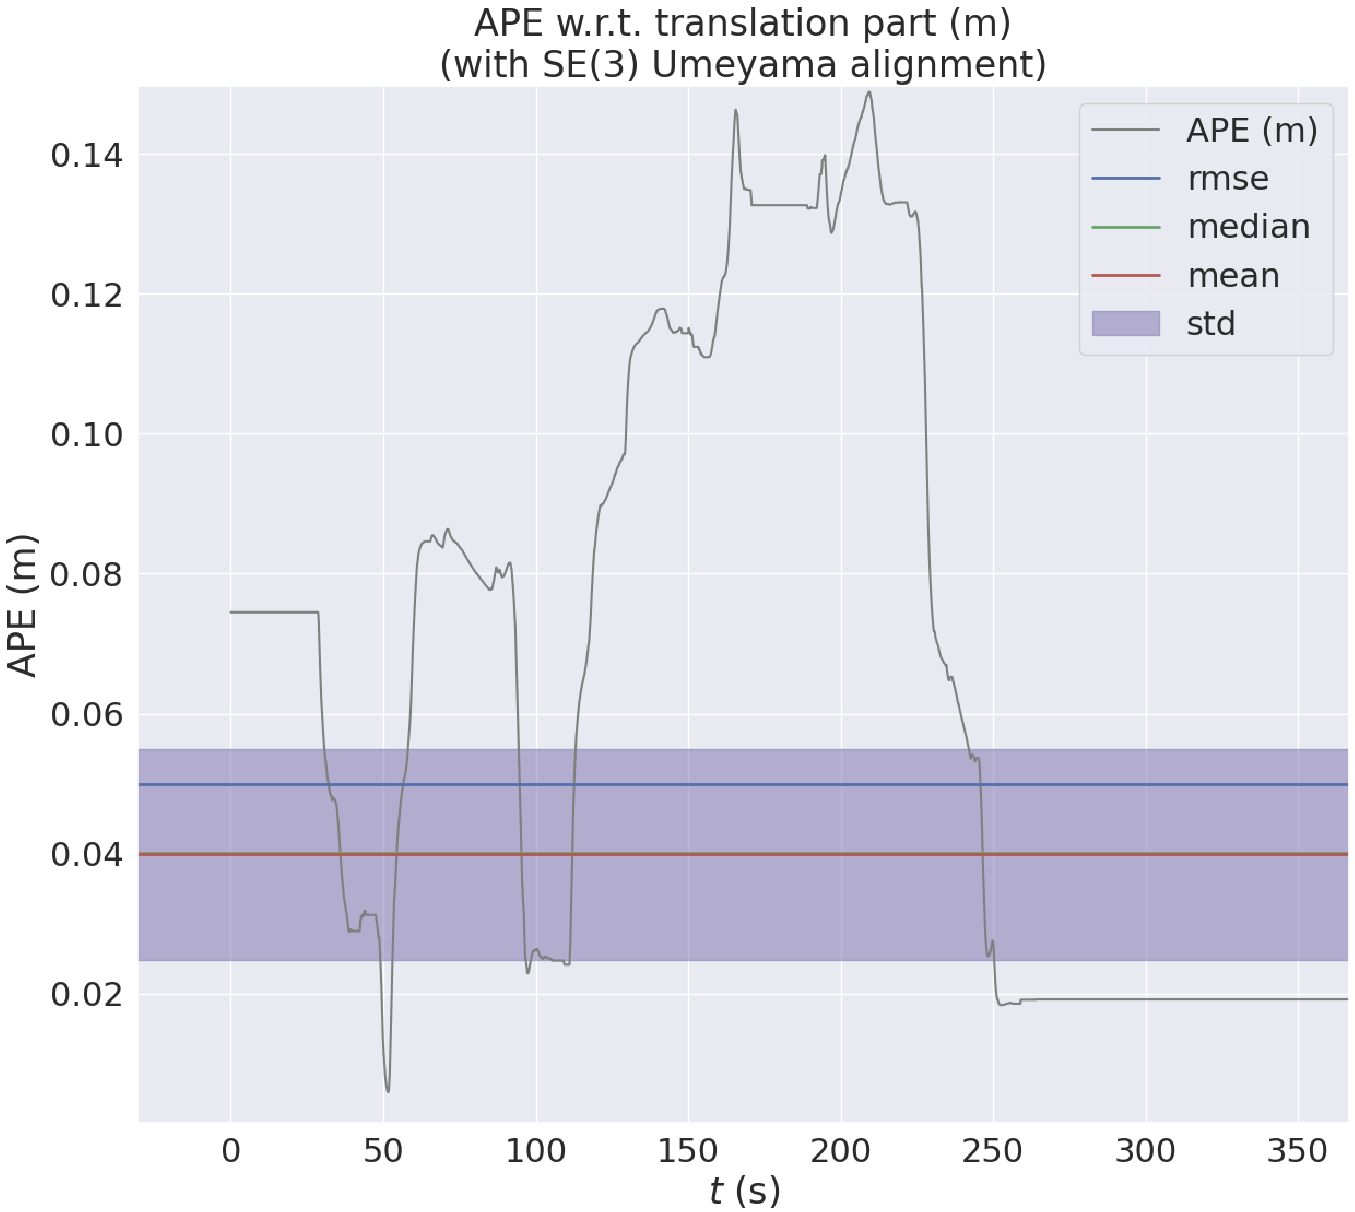
\includegraphics[width=.48\linewidth]{images/APE_graph.png}}\hfill
        \subfloat[ATE values over the map]{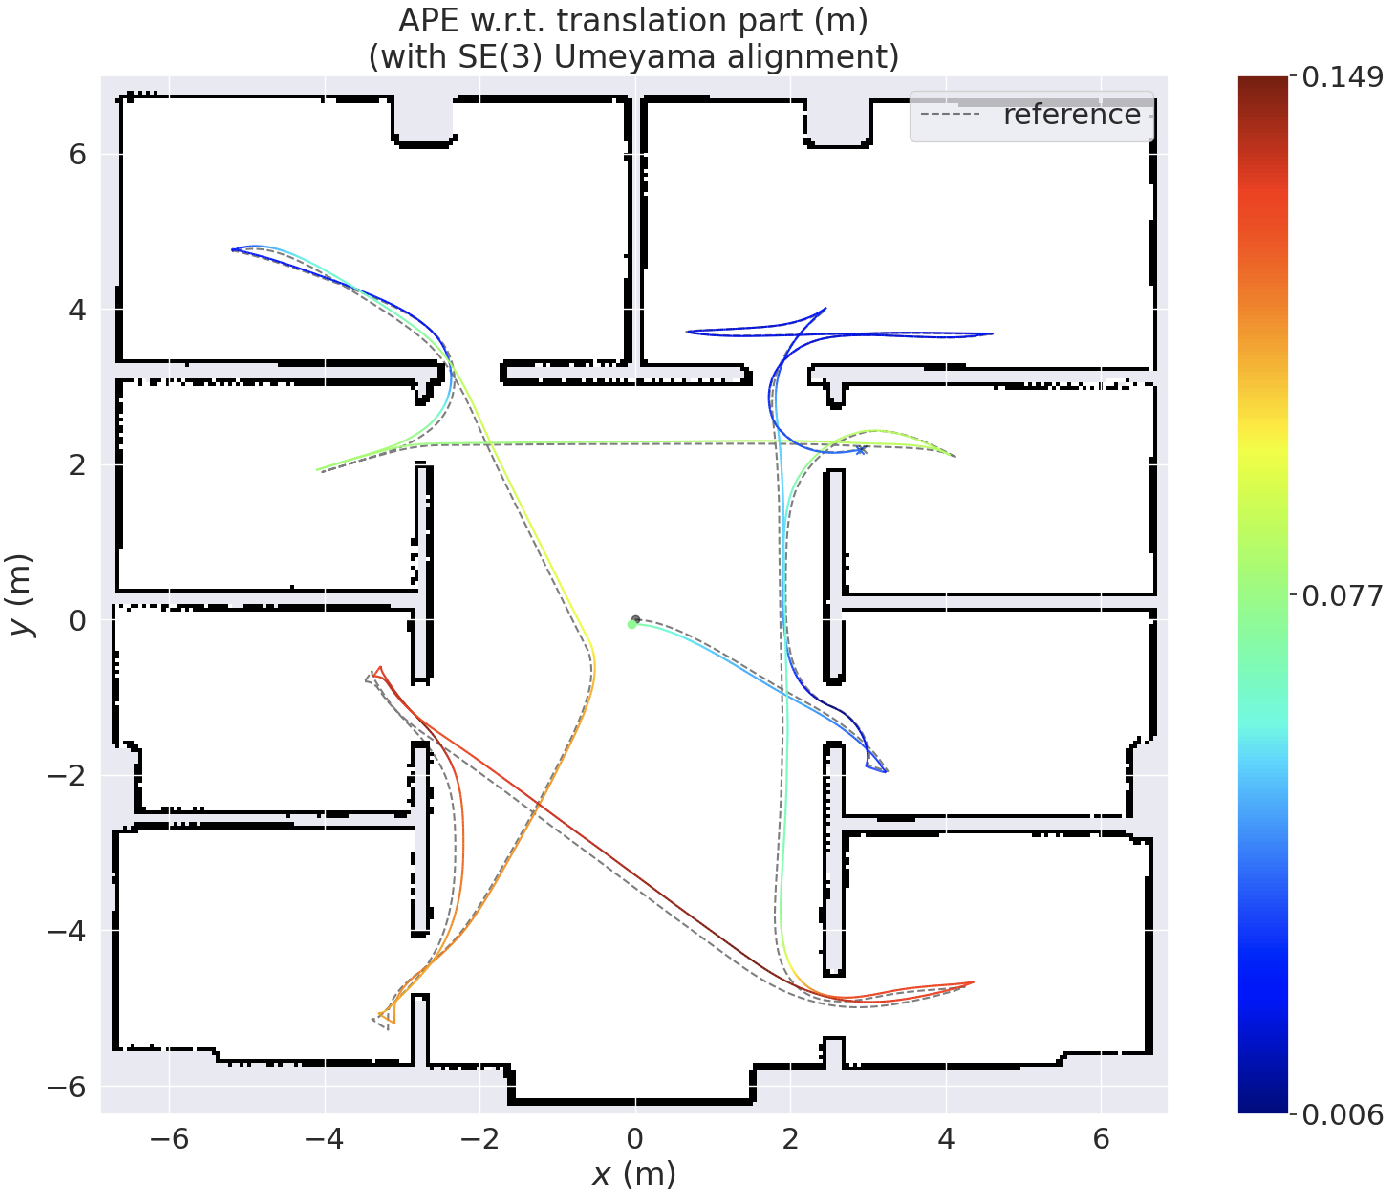
\includegraphics[width=.5\linewidth]{images/APE_map.png}}
    \caption{Visualizations of ATE variations during exploration, realized with \textit{evo}\protect\footnotemark.}\label{fig:APE_graphs}
    \end{figure}
\footnotetext{https://github.com/MichaelGrupp/evo}

\noindent
In order to compute ATE and ARE values after a robot has explored an environment, we need to compare all the pairs of key-points sampled from the estimated trajectory of the robot and its ground truth (GT) trajectory. Specifically, during exploration we sample $T$ poses, where each pose is a vector containing the position and orientation of the robot, and we build two sets $x_{1:T}$, $x_{1:T}^*$ that contain, respectively, the estimated and GT poses. \\
Next, we define $\delta_{i,j} = x_j\ominus x_i$ as the relative transformation\footnote{Which is a transformation matrix that describes a rigid transform.} that moves the robot from pose $x_i$ to $x_j$, and its counterpart $\delta_{i,j}^* = x_j^*\ominus x_j^*$. Then we define the $trans(\cdot)$ and $rot(\cdot)$ functions which extract, respectively, the translational component of a transform (i.e., a vector $z_{ij}\in\mathbb{R}^2$ representing the translation delta needed to move from pose i to j) and the rotational component (i.e., a vector $\theta_{ij}\in\mathbb{R}^2$ that expresses the angular deltas as Euler angles).
Finally, to compute the localization error we consider all sorted pairs of transformations $\{\delta_{i,j} : j < i, \forall i\in2\dots T\}$:

\begin{equation*}
    \begin{split}
        \centering
            \varepsilon(\delta) & = \varepsilon_t(\delta) + \varepsilon_r(\delta)\\
            & = \frac{1}{N}\sum_{i, j}trans(\delta_{i,j}\ominus\delta_{i,j}^*)+\frac{1}{N}\sum_{i, j}rot(\delta_{i,j}\ominus\delta_{i,j}^*)\\
            & = \frac{1}{N}\sum_{i, j}(||z_{ij} - z_{ij}^*||_2 + ||\theta_{ij} - \theta_{ij}^*||_2) \\
            & = \frac{2}{(T-1)^2}\sum_{i=2}^T\sum_{j=1}^{i-1}(||z_{ij} - z_{ij}^*||_2 + ||\theta_{ij} - \theta_{ij}^*||_2)\\
    \end{split}
\end{equation*}

\noindent
Note that these metrics are dependent on the availability of the GT data, which is easily obtained in simulated environments but extremely difficult to obtain when deploying a robot in the real world, as it would require an external system to accurately track its real position.

% -----------------------------------------------------------
%                                                           \
%                                                           \
% -----------------------------------------------------------

\subsection{Task formulation} % -------------------------------------------------------
\noindent
Calculating the localization error is usually performed after the robot has explored an environment, thus a full re-exploration is required in case the SLAM process yields poor results. Having an \textit{a-priori} prediction of the localization error of a certain environment can be used to preemptively adjust the sensor equipment or the SLAM algorithm used by the robot.

To address these limitations, the work in \cite{luperto2021predicting}, proposes a method to perform an \textit{a-priori} prediction of the expected ATE and ARE, based on the geometric/topological characteristics of an indoor environment: using a feature extractor, described in \cite{luperto2019extracting}, a set of structural features is extracted from a floorplan, in order to represent each environment as a vector $v\in\mathbb{R}^k$, where $k$ is the number of distinct features.
Successively, each environment is explored by a simulated robot, and, by collecting both GT and estimated trajectories, the corresponding ATE and ARE are computed and stored.

\noindent
Finally, two models are trained on this dataset:
\begin{itemize}
    \item \textbf{Linear model:} computed using linear regression.
    \item \textbf{Gaussian Process:} computed using an RBF kernel.\\
\end{itemize}
\noindent
The goals of this project are the following:
\begin{enumerate}
    \item Evaluate how multiple predictors, based on state-of-the-art convolutional neural networks (CNN), perform with respect to the linear and Gaussian models. In particular, with the usage of a CNN, it is possible to delegate the feature extraction stage to the network itself, so that a floorplan's image can be fed directly to the model, without computing a set of hand-crafted features.
    \item Automatically handle model selection by delegating both hyperparameter optimization and neural architecture search to an optimization framework.
\end{enumerate}


\noindent
Each environment in our dataset is represented as a floorplan image and has three associated quantities: area ($m^2$), ATE ($m$), and ARE ($rad$). The predictor we want to build takes as input the floorplan image, together with the area, and produces two values in output, corresponding to the predicted ATE and ARE values.

\noindent
More formally, the model $h$ we want to learn can be expressed as follows:
$$
    h: X \rightarrow Y\ ,\ X\in (Mat_{n \times n}\times\mathbb{R}),\ Y\in\mathbb{R}^2 
$$